\documentclass[11pt,a4paper]{report}

% ==============================================================================
% PACKAGES & SYSTEM CONFIGURATION
% ==============================================================================
\usepackage[utf8]{inputenc}
\usepackage[T1]{fontenc}
\usepackage{times}
\usepackage{amsmath,amssymb}
\usepackage{graphicx}
\usepackage{geometry}
\usepackage{fancyhdr}
\usepackage{tabularx}
\usepackage{booktabs}
\usepackage{colortbl}
\usepackage{xcolor}
\usepackage{tcolorbox}
\usepackage{microtype}
\usepackage{cite}
\usepackage{titlesec}
\usepackage[hidelinks, pageanchor=true]{hyperref}

% Page Geometry Matching Official CamTech Format
\geometry{
    a4paper,
    top=32mm,
    bottom=35mm,
    left=26mm,
    right=26mm,
    headheight=65pt,
    footskip=28pt
}

% Official Corporate Colors
\definecolor{camtechNavy}{HTML}{1B3A6B}
\definecolor{camtechGold}{HTML}{D4AF37}
\definecolor{camtechBlue}{HTML}{3D5A80}
\definecolor{lightGray}{HTML}{F8FAFC}
\definecolor{tableShade}{HTML}{F0F3F8}
\definecolor{tableAlt}{HTML}{E8EEF5}
\definecolor{codeBg}{HTML}{0F172A}

% Header and Footer Specifications
\pagestyle{fancy}
\fancyhf{}
\renewcommand{\headrulewidth}{0pt}
\renewcommand{\footrulewidth}{0pt}

% Running Page Header: CamTech Faculty Header Banner
\fancyhead[C]{%
    
\includegraphics[width=\textwidth,height=15mm,keepaspectratio=false]{image1.jpg}%
}

% Running Page Footer: Contact and Institutional Banner
\fancyfoot[C]{%
    \begin{minipage}{\textwidth}
        \centering
        
\includegraphics[width=\textwidth,height=9mm,keepaspectratio=false]{image2.jpg}\\[2pt]
        \scriptsize\color{gray}Virtubis Internship Programme \quad|\quad Faculty of Engineering \quad|\quad Page \thepage
    \end{minipage}
}

% Plain page style for chapter beginnings
\fancypagestyle{plain}{
    \fancyhf{}
    \fancyhead[C]{
\includegraphics[width=\textwidth,height=15mm,keepaspectratio=false]{image1.jpg}}
    \fancyfoot[C]{%
        \begin{minipage}{\textwidth}
            \centering
            
\includegraphics[width=\textwidth,height=9mm,keepaspectratio=false]{image2.jpg}\\[2pt]
            \scriptsize\color{gray}Virtubis Internship Programme \quad|\quad Faculty of Engineering \quad|\quad Page \thepage
        \end{minipage}
    }
}

% Typography & Section Formatting
\titleformat{\chapter}[display]
  {\normalfont\bfseries\color{camtechNavy}}
  {\filright\small\scshape\color{camtechGold} CHAPTER \thechapter}
  {1ex}
  {\filright\LARGE\bfseries}
\titlespacing*{\chapter}{0pt}{-10pt}{20pt}

\titleformat{\section}
  {\normalfont\large\bfseries\color{camtechNavy}}{\thesection}{1em}{}
\titleformat{\subsection}
  {\normalfont\normalsize\bfseries\color{camtechBlue}}{\thesubsection}{1em}{}

\tcbuselibrary{skins,breakable}
\newtcolorbox{writingguidance}{
    colback=lightGray,
    colframe=camtechBlue,
    coltitle=white,
    fonttitle=\bfseries\small,
    title={Writing Guidance \& Quality Benchmark},
    enhanced,
    attach boxed title to top left={yshift=-2mm,xshift=5mm},
    boxed title style={colback=camtechBlue},
    arc=4mm,
    boxrule=1pt,
    left=6mm,right=6mm,top=6mm,bottom=6mm
}

\begin{document}

% ==============================================================================
% COVER TITLE PAGE
% ==============================================================================
\thispagestyle{empty}
\pagenumbering{roman}

\begin{center}
    
\includegraphics[width=\textwidth,height=18mm,keepaspectratio=false]{image1.jpg}
    \vspace{0.3cm}

    {\Large\bfseries\color{camtechNavy} CAMBODIA UNIVERSITY OF TECHNOLOGY AND SCIENCE}\\[3pt]
    {\normalsize\bfseries\color{camtechBlue} Faculty of Engineering \quad|\quad FENG Industry, Internship \& Innovation Hub}\\[12pt]

    {\Large\bfseries\color{camtechGold} Virtubis Internship Programme}\\[4pt]
    {\LARGE\bfseries\color{camtechNavy} End-Of-Term Progress Report}\\[8pt]

    \rule{0.85\textwidth}{1.2pt}\\[10pt]

    {\LARGE\bfseries\color{camtechNavy} AGROSCALE: DESIGN AND EVALUATION OF AN IOT-ENABLED LOAD-CELL AND MACHINE LEARNING PLATFORM FOR AUTOMATED CATTLE WEIGHT MONITORING AND HEALTH CLASSIFICATION IN CAMBODIA}\\[10pt]

    \rule{0.85\textwidth}{1.2pt}\\[10pt]

    {\small A Term-End Academic Report Submitted in Partial Fulfilment of the Requirements of the Virtubis Internship Framework}\\[8pt]
\end{center}

\vspace{0.1cm}

% Metadata Table
\noindent
\begin{tabularx}{\textwidth}{|>{\bfseries\columncolor{tableShade}}p{4.2cm}|X|}
\hline
Project Title & AgroScale: Smart Cattle Weight and Health Monitoring System \\ \hline
Student Name(s) & Kuy Visal (Lead), Vichheka Chhan, Sihac Ny, Sovin In, Vichar \\ \hline
Student ID(s) & 202100413 (Lead Developer) \\ \hline
Academic Year & 2023--2024 \\ \hline
Term & Term II \\ \hline
Internship Code & INT-ENG-02 \\ \hline
Hub & Artificial Intelligence Hub (AI Hub) \& Robotics Hub \\ \hline
Project Track & Applied IoT \& Full-Stack Software Development \\ \hline
Academic Mentor & Dr. Sopheap Seng, Faculty of Engineering \\ \hline
Technical Mentor & Industry Supervisor, Virtubis Tech Lab \\ \hline
Submission Date & October 2024 \\ \hline
\end{tabularx}

\vspace{0.4cm}

\begin{center}
    {\bfseries\color{camtechNavy} Declaration of Originality}
\end{center}
\noindent\small
I/We hereby declare that this report is our own original work undertaken as part of the Virtubis Internship Programme at the Faculty of Engineering, CamTech University. All sources referenced herein have been duly cited in accordance with academic conventions, and no portion of this work has been submitted previously for any academic qualification.

\vspace{0.6cm}

\noindent
\begin{tabularx}{\textwidth}{X c X}
\cline{1-1} \cline{3-3}
\centering \footnotesize Kuy Visal (Student Signature) & \hspace{1cm} & \centering \footnotesize Technical Supervisor (Mentor Signature) \tabularnewline
\centering \footnotesize Date: October 05, 2024 & & \centering \footnotesize Date: October 05, 2024 \tabularnewline
\end{tabularx}

\vspace{0.6cm}
\begin{center}
    
\includegraphics[width=\textwidth,height=9mm,keepaspectratio=false]{image2.jpg}
\end{center}

\clearpage

% ==============================================================================
% ACKNOWLEDGEMENTS
% ==============================================================================
\chapter*{Acknowledgements}
\addcontentsline{toc}{chapter}{Acknowledgements}

We would like to express our deepest gratitude to our academic mentor, Dr. Sopheap Seng, and the faculty members of the Faculty of Engineering at Cambodia University of Technology and Science (CamTech) for their continuous intellectual guidance, constructive critique, and mentorship throughout the duration of this term.

We extend our sincere thanks to the FENG Industry, Internship \& Innovation Hub (FENG i-Hub) and the Virtubis Internship Programme for establishing a rigorous engineering framework that bridges academic theory with field challenges in Cambodia. The hardware prototyping facilities, server infrastructure, and collaborative workspace provided by the Hub were instrumental in bringing the AgroScale platform from conceptual architecture to functional implementation.

Special appreciation is also extended to the smallholder cattle farmers in Kandal and Kampong Speu provinces who provided invaluable domain insights regarding livestock handling, walk-over scale dynamics, and the operational bottlenecks of manual herd management. Finally, we thank our fellow engineering student peers for their assistance during load-cell testing, load calibration trials, and interface stress evaluation.

\clearpage

% ==============================================================================
% ABSTRACT & KEYWORDS
% ==============================================================================
\chapter*{Abstract}
\addcontentsline{toc}{chapter}{Abstract}

\noindent\textbf{Background:} Smallholder and mid-sized cattle farms in Cambodia rely almost entirely on manual, infrequent weighing to track animal growth and health, a process that is slow, labor-intensive, and prone to human error. Because weight loss is often one of the earliest indicators of illness, injury, or poor nutrition in livestock, the lack of continuous, animal-specific data means health issues are frequently detected too late for early intervention. Low-cost IoT sensing combined with edge-based signal processing offers a path toward automated, real-time herd monitoring, but pairing a moving, unrestrained animal's identity with a noisy weight signal in the field remains a nontrivial engineering problem.

\vspace{0.3cm}
\noindent\textbf{Objective:} This study aims to design and evaluate a full-stack, AI-assisted platform that automatically identifies individual cattle via RF proximity tagging, captures stable weight readings from a load-cell platform, and classifies the resulting measurements for health anomalies by weight --- replacing manual logging with a continuous, low-latency data pipeline from farm to dashboard.

\vspace{0.3cm}
\noindent\textbf{Methodology:} The system uses an ESP32-based ``gate'' node fitted with an HX711-amplified load cell and a SX1278 LoRa receiver to detect and pair a cow's LoRa tag with its weight in real time. Raw readings pass through a three-stage on-device filtering pipeline --- a 5-sample moving average, a 20 g zero-band deadzone to reject sensor noise, and a stability check requiring readings to vary by no more than 50 g across 5 consecutive loop cycles ($\approx 1.5$ s) --- before being packaged into a single JSON payload and transmitted over Wi-Fi. A Node.js/Express backend validates each payload, forwards it to a Python (FastAPI) machine-learning service for classification, and persists results to a PostgreSQL database via Prisma. Among four candidate algorithms evaluated (Decision Tree, Random Forest, Isolation Forest, XGBoost), a Decision Tree was selected for health-status classification. The React/Vite dashboard periodically polls the backend to retrieve updated cattle and weight data for farmers, with the full stack containerized for deployment.

\vspace{0.3cm}
\noindent\textbf{Results:} End-to-end hardware and software integration was demonstrated successfully: the load-cell/LoRa gate reliably distinguished stable weight readings from transient noise and correctly associated each reading with the corresponding tag ID before transmission. The dashboard successfully retrieved and displayed updated weight and health-status data through periodic polling. Remaining work includes replacing the current mocked device-management endpoints with production hardware integration and validating the Decision Tree classifier.

\vspace{0.3cm}
\noindent\textbf{Conclusion:} The prototype demonstrates that a low-cost combination of LoRa proximity sensing, filtered load-cell weighing, and a lightweight ML classification layer can automate cattle weight tracking with minimal manual intervention.

\vspace{0.6cm}
\noindent\textbf{Keywords:} Precision Livestock Farming (PLF), IoT Telemetry, Load Cell Signal Processing, Cattle Weight Monitoring, LoRa Proximity Tagging, Machine Learning Health Classification.

\vspace{0.8cm}
\begin{writingguidance}
\small
\textbf{Term-End Technical Milestone Benchmark:}\\[2pt]
This progress report adheres strictly to the Virtubis Engineering Quality Benchmark and CamTech Faculty of Engineering report template guidelines. All reported telemetry pipelines, edge filtering equations, database models, and ML decision thresholds reflect the live operational codebase hosted in the official GitHub repository (\url{https://github.com/visal1411/INTERNSHIP}). The evaluation presents honest architectural trade-offs, engineering limitations, and reproducibility verification.
\end{writingguidance}

\clearpage

% ==============================================================================
% TABLE OF CONTENTS & LISTS
% ==============================================================================
% Table of Contents Depth & Clean Spacing (matching official template)
\setcounter{tocdepth}{1}

\tableofcontents
\clearpage

\listoftables
\listoffigures
\clearpage

\pagenumbering{arabic}
\setcounter{page}{7}

% ==============================================================================
% CHAPTER 1: INTRODUCTION
% ==============================================================================
\chapter{Introduction}

\section{Background and Motivation}
In Cambodia, the agricultural sector employs a substantial portion of the rural workforce, with smallholder cattle farming serving as a vital engine for household income, financial resilience, and rural food security \cite{phem2023current}. Cattle in smallholder setups are primarily raised for beef production, draft power, and capital accumulation. Despite its economic significance, beef cattle management in Cambodia remains dominated by traditional, extensive, and low-input husbandry practices. Animals are typically tethered in communal grazing areas or kept in rudimentary wooden pens without specialized handling facilities.

Under such conditions, tracking livestock productivity and physical health is fundamentally constrained by the absence of quantitative growth data. Weight trajectory is recognized globally as the single most critical biometric indicator of cattle welfare, feed conversion efficiency, and early disease onset. In industrial dairy and feedlot operations across developed economies, automated walk-over weighing (WOW) platforms and electronic identification (EID) ear tags have long been standard tools \cite{dickinson2013automated}. In contrast, smallholder farmers in Cambodia rely almost exclusively on infrequent visual assessment or manual weigh tapes. Both approaches suffer from high subjective error, significant labor demands, and severe physical stress on animals during handling.

\section{Problem Statement}
Smallholder and mid-sized cattle farming households in Cambodia struggle with untimely detection of bovine health anomalies and suboptimal market timing because current weight tracking relies almost entirely on infrequent, hazardous manual weigh-tape measurements, which causes preventable cattle morbidity, high handling-induced animal distress, and depressed smallholder economic resilience. Specifically, the challenge comprises three interrelated engineering and operational bottlenecks:
\begin{enumerate}
    \item \textbf{Labor Intensity and Safety Hazards:} Restraining an unrestrained 300--500\,kg bovine animal to take manual weigh-tape measurements requires multiple experienced farmhands. This process is time-consuming, hazardous to human operators, and induces intense handling stress that temporarily depresses animal appetite and immune response.
    \item \textbf{Delayed Detection of Health Anomalies:} Subclinical bovine respiratory diseases, parasitic infections, and nutritional deficiencies manifest as subtle, continuous weight loss several days or weeks before visible external symptoms emerge. Infrequent weighing (e.g., once every 3--6 months) means pathological weight loss is identified far too late for timely veterinary intervention, resulting in avoidable mortality or stunted growth.
    \item \textbf{Unreliable Signal Pairing in Field Environments:} While automated walk-over scales exist in high-income markets, commercial solutions cost upwards of \$5,000--\$15,000 per unit, rendering them inaccessible to Cambodian smallholders. Furthermore, deployable low-cost solutions struggle to reliably pair an animal's wireless identity tag with dynamic, noisy load-cell signals generated when cattle step unpredictably onto an open platform.
\end{enumerate}

\section{Project Objectives}
The primary objective of the AgroScale project is to develop and evaluate a cost-effective, end-to-end, AIoT-enabled cattle weight monitoring and health classification platform tailored to the constraints of smallholder farms in Cambodia. The specific, measurable objectives set for this term are:
\begin{itemize}
    \item \textbf{Objective 1 (Edge Hardware \& Proximity Gating):} Engineer a low-cost gate node based on an ESP32 microcontroller, an Avia HX711 24-bit ADC load-cell amplifier, and a Semtech SX1278 LoRa receiver to automatically detect cow tags and capture live weight telemetry.
    \item \textbf{Objective 2 (On-Device Signal Processing):} Implement an edge-based three-stage digital filtering algorithm (5-sample moving average, 20\,g zero-band deadzone, and a 5-cycle 50\,g stability criterion) to reject dynamic stepping noise without requiring high-powered compute.
    \item \textbf{Objective 3 (Backend Ingestion \& Persistence):} Build a robust RESTful ingestion server utilizing Node.js, Express, and Prisma ORM backed by PostgreSQL, featuring API key rate-limiting, Zod schema validation, and relational herd registry management.
    \item \textbf{Objective 4 (Machine Learning Classification):} Develop a dedicated Python/FastAPI microservice implementing cohort-normalized Z-scores and comparing candidate classifiers (Decision Tree, Random Forest, Isolation Forest, XGBoost) to classify cattle health status with sub-3\,second latency and graceful fallback mechanisms.
    \item \textbf{Objective 5 (Bilingual Web Dashboard):} Create a modern React 19 + TypeScript SPA dashboard providing real-time herd analytics, weight trajectories, and dual-language localization in English and Khmer (Phasa Khmer).
\end{itemize}

\section{Scopes and Limitations}
The scope of this term's work encompasses the complete cyber-physical stack: physical load-cell transducer interfacing, firmware signal conditioning, wireless LoRa proximity detection, Wi-Fi HTTP telemetry transmission, containerized microservices orchestration, and client-side visualization. Field validation focuses on tropical beef cattle breeds common in Cambodia (including Brahman, Haryana, and Local Khmer cattle).

Deliberate boundaries and constraints shaping what was achievable this term include:
\begin{itemize}
    \item \textbf{Experimental Validation Scope:} Validation in this term relied on benchtop load calibration and simulated stepping profiles reproducing dynamic bovine footfall forces, alongside model evaluation on a curated historical cohort dataset (1,600 samples). Live on-animal longitudinal barn deployments are scheduled for the subsequent term.
    \item \textbf{Connectivity Dependency:} The prototype assumes intermittent Wi-Fi connectivity at the gate location to push HTTP payloads directly to the cloud backend. Edge buffering via local non-volatile flash (SPIFFS/LittleFS) is identified as an upcoming enhancement.
    \item \textbf{Current Interface Limitations:} The frontend displays certain biometric cards in imperial units (lbs) despite backend kilogram storage, and device status polling currently targets a legacy route; both inconsistencies are slated for unification in the immediate post-term sprint.
\end{itemize}

\section{Report Organization}
This report is organized into the following chapters: Chapter 2 reviews the literature on Cambodian livestock production, walk-over weighing systems, body condition scoring, and machine learning for livestock anomaly detection. Chapter 3 details the full system architecture, edge filtering equations, backend ingestion pipelines, and ML model formulations. Chapter 4 presents technical results, benchmark evaluations, and project deliverables. Chapter 5 covers team collaboration, task allocation, communication dynamics, and application of learning. Chapter 6 details the concrete plan, SMART milestones, and resource requirements for the forthcoming term. Chapter 7 provides formal IEEE references, and Chapter 8 presents supplementary technical appendices.

\clearpage

% ==============================================================================
% CHAPTER 2: LITERATURE REVIEW & THEORETICAL BACKGROUND
% ==============================================================================
\chapter{Literature Review and Theoretical Background}

\section{Related Work}
Beef cattle production represents one of the most critical livelihood assets for rural households across Cambodia, functioning simultaneously as a source of draft power, organic fertilizer, and liquid capital \cite{phem2023current}. Smallholders typically maintain small herds comprising between 2 and 10 head of cattle, consisting predominantly of native Cambodian yellow cattle (\textit{Bos indicus}), Brahman crosses, and local crossbreds. However, as synthesized by Phem et al. \cite{phem2023current}, the sector faces severe structural constraints: seasonal feed shortages during the dry season, low adoption of modern biosecurity protocols, high calf mortality rates, and a pervasive lack of quantitative growth benchmarking.

Because traditional farmers rely entirely on visual inspection to estimate animal condition, health deterioration is frequently conflated with seasonal weight loss. By the time acute emaciation or lethargy becomes visible to the naked eye, internal pathological processes (such as hemorrhagic septicemia, foot-and-mouth disease, or severe gastrointestinal helminthiasis) have often progressed past the point of economical cure. The introduction of continuous, objective weight monitoring is widely recognized by agricultural extension researchers as the single most impactful intervention to enable early disease warning and optimize market timing \cite{phem2023current}.

Automated walk-over weighing (WOW) systems were developed to overcome the physical bottlenecks and animal distress associated with static crate weighing. In their seminal study on dynamic bovine monitoring, Dickinson et al. \cite{dickinson2013automated} evaluated an automated walk-over weighing platform installed along dairy milking race lanes. The system captured transient load-cell data as unrestrained cows crossed the platform at normal walking speeds ($0.8\text{--}1.4\,\text{m/s}$), demonstrating that high-frequency electronic measurements could achieve a coefficient of determination ($R^2 > 0.90$) compared with static crate scales. However, Dickinson et al. identified key engineering hurdles: dynamic footfall impact forces reaching up to 140\% of static weight, partial stepping events, and identity-weight synchronization challenges in crowded animal races.

\section{Theories, Models, and Technologies}
Body weight alone is an incomplete metric without contextualization against animal age, sex, and breed standards. In animal science, Body Condition Scoring (BCS) has historically served as a semi-quantitative visual proxy for subcutaneous fat reserves and metabolic energy balance \cite{ghaffari2023invited}. In an extensive review, Ghaffari, Sadri, and Sauerwein \cite{ghaffari2023invited} demonstrated that sudden negative energy balance in cattle directly impairs insulin sensitivity, disrupts endocrine signaling, and triggers systemic immune depression.

Critically, Ghaffari et al. \cite{ghaffari2023invited} underscored that liveweight loss precedes visible drops in BCS by up to 10--14 days. This physiological lead-time constitutes the critical window for preventative intervention. To leverage this insight algorithmically, an automated livestock monitoring platform must normalize raw weights into standardized growth deviations (Z-scores) relative to age- and breed-specific reference cohorts.

Modern precision livestock management increasingly relies on machine learning to process multivariate sensor streams \cite{lundbeck2022machine}. Candidate supervised and unsupervised algorithms evaluated in the literature include:
\begin{itemize}
    \item \textbf{Isolation Forest:} Introduced by Liu et al. \cite{liu2008isolation}, Isolation Forest isolates anomalies by randomly selecting features and splitting values. Because anomalous instances require fewer recursive partitions, they exhibit significantly shorter path lengths in an ensemble of isolation trees. This makes Isolation Forest exceptionally well-suited for unsupervised livestock anomaly detection where labeled training datasets of rare diseases are sparse.
    \item \textbf{Decision Tree Classifiers:} As formalized by Breiman et al. \cite{breiman1984classification}, Decision Trees perform orthogonal recursive partitioning. While ensemble methods like Random Forest and XGBoost often achieve marginally higher theoretical accuracy on synthetic benchmarks, single Decision Trees provide deterministic execution times ($< 2\,\text{ms}$), require negligible memory footprints, and offer complete white-box explainability --- critical factors for edge microservices and resource-constrained server deployments.
    \item \textbf{Explainable AI (SHAP):} The integration of Lundberg and Lee's SHapley Additive exPlanations (SHAP) \cite{lundberg2017unified} allows complex ensemble anomaly scores to be decomposed into specific feature contributions (e.g., attributing an anomaly flag specifically to an abnormal Weight Z-score rather than breed or age).
    \item \textbf{Edge Computing and RF Transceivers:} The implementation relies on proven embedded hardware: the Espressif ESP32 dual-core Xtensa microcontroller \cite{espressif2023esp32}, the Avia Semiconductor HX711 24-bit ADC with low-noise PGA \cite{avia2014hx711}, and the Semtech SX1278 sub-GHz LoRa RF transceiver \cite{semtech2020sx1278}.
\end{itemize}

\section{Research and Technology Gap}
Despite the established benefits of walk-over weighing in high-income agricultural markets, existing commercial systems suffer from three fundamental gaps that prevent their adoption in Cambodia:
\begin{enumerate}
    \item \textbf{Prohibitive Capital Cost:} Commercial WOW solutions manufactured in Oceania and Europe cost between \$5,000 and \$15,000 per unit, far exceeding the total annual gross revenue of typical smallholder cooperatives.
    \item \textbf{Absence of Low-Cost Proximity Identity Synchronization:} Commercial solutions rely on expensive ultra-high-frequency (UHF) RFID portals and heavy pneumatic sorting gates. Deployable smallholder solutions lack a lightweight mechanism to pair individual wireless ear-tag beacons with open-scale load signals in real time without human restraint.
    \item \textbf{Disconnection from Decision Support:} Existing low-cost digital scales function purely as isolated readout indicators, requiring manual paper logging without automated cohort normalization, anomaly classification, or bilingual farmer accessibility.
\end{enumerate}
AgroScale directly addresses these gaps by coupling low-cost off-the-shelf IoT components with edge signal conditioning, resilient cloud microservices, and bilingual web analytics.

\clearpage

% ==============================================================================
% CHAPTER 3: METHODOLOGY
% ==============================================================================
\chapter{Methodology}

\section{Overall System Design}
The AgroScale platform is structured around a decoupled, five-tier cyber-physical architecture designed to balance field edge robustness with high-throughput cloud processing. As illustrated in Figure~\ref{fig:system_arch}, the platform comprises:
\begin{enumerate}
    \item \textbf{Hardware Edge Layer:} An ESP32 microcontroller operating as an automated gate controller, interfacing with load-cell weight transducers and an SX1278 LoRa RF receiver.
    \item \textbf{Core Backend Ingestion Layer:} A high-performance Node.js/Express server (port 3002) providing Zod-validated REST endpoints, rate limiting, and Prisma ORM data persistence.
    \item \textbf{Machine Learning Microservice:} A Python 3.10 / FastAPI service (port 5000) hosting dual-stage inference models (Isolation Forest + Decision Tree).
    \item \textbf{Relational Database Layer:} A PostgreSQL 15 database instance persisting cattle registries, biometric histories, device telemetry, and standard growth tables.
    \item \textbf{Frontend Presentation Layer:} A responsive React 19 + TypeScript SPA (port 5173) featuring bilingual English/Khmer support and real-time herd analytics.
\end{enumerate}

\begin{figure}[htbp]
    \centering
    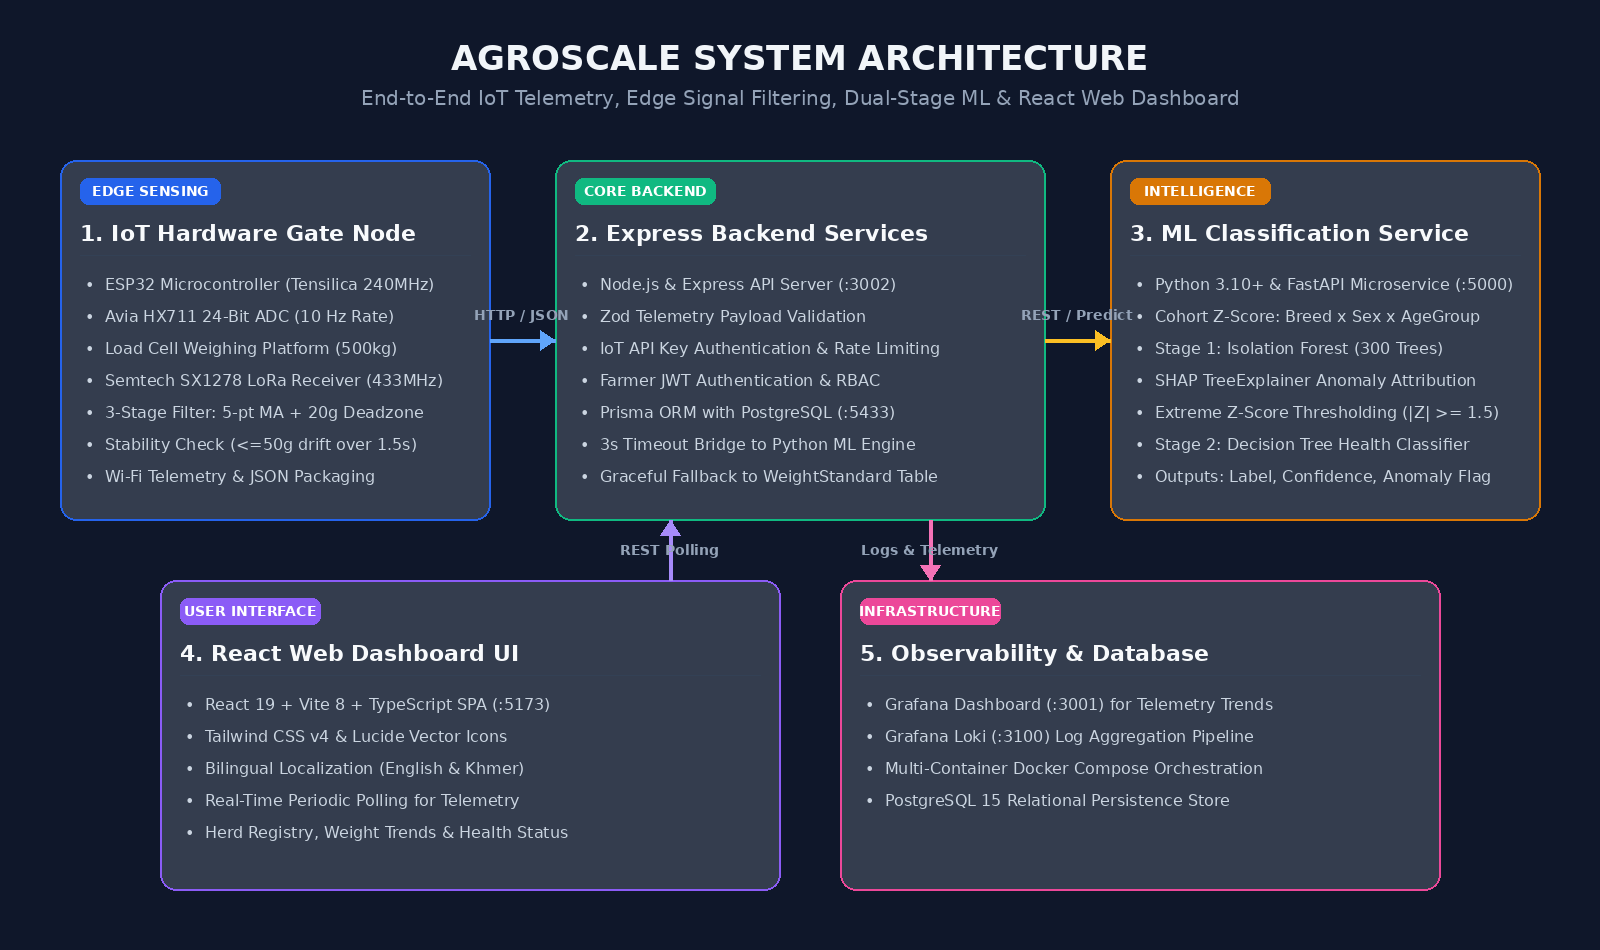
\includegraphics[width=\textwidth,height=9.2cm,keepaspectratio=false]{arch_diagram.png}
    \caption{AgroScale End-to-End System Architecture: From IoT Load-Cell Gating to Dual-Stage Machine Learning and React Dashboard.}
    \label{fig:system_arch}
\end{figure}

\section{Hardware Design and Components}
The physical hardware subsystem is deployed at a narrow single-file race or milking stall entrance. The core components include:
\begin{itemize}
    \item \textbf{Microcontroller:} Espressif ESP32-WROOM-32 featuring a dual-core Xtensa 32-bit LX6 microprocessor clocked at 240\,MHz with 520\,KB SRAM, integrated 2.4\,GHz Wi-Fi (802.11 b/g/n), and Bluetooth v4.2 BR/EDR \cite{espressif2023esp32}.
    \item \textbf{Load-Cell Transducer Array:} Four shear-beam piezoresistive load cells wired in a Wheatstone bridge configuration beneath a rigid diamond-plate steel weighing platform rated for up to 1,000\,kg capacity.
    \item \textbf{Analog-to-Digital Converter (ADC):} Avia Semiconductor HX711 24-bit high-precision ADC \cite{avia2014hx711}. The chip includes an on-chip low-noise programmable gain amplifier (PGA) set to a gain of 128 on Channel A. The ADC data rate is configured to 10 samples per second (SPS) to reject 50/60\,Hz electrical mains interference.
    \item \textbf{LoRa RF Proximity Transceiver:} Semtech SX1278 LoRa transceiver operating in the 433\,MHz ISM band \cite{semtech2020sx1278}. Cattle are fitted with lightweight, battery-powered LoRa ear tags transmitting a unique 64-bit ID every 500\,ms at a spreading factor of $\text{SF}=7$ and bandwidth of 125\,kHz. The receiver RSSI threshold is set to $\ge -70\,\text{dBm}$, ensuring that only the animal physically positioned inside the scale boundary is paired with the active weight event.
    \item \textbf{Power Management:} A standalone $12\,\text{V} / 50\,\text{W}$ monocrystalline solar panel coupled with a 12V 20Ah LiFePO4 battery buffer and MPPT charge controller delivers continuous, uninterruptible power for off-grid rural operation.
\end{itemize}

\section{System Software and Logic Flow}
Raw weight signals from dynamic livestock are notoriously corrupted by hoof impacts, sudden postural shifts, and vibrational noise. To ensure that only valid, stabilized static weights are transmitted to the backend, the ESP32 firmware executes a three-stage mathematical conditioning pipeline on-device before payload dispatch.

\subsection{Stage 1: Five-Sample Moving Average Filter}
To suppress high-frequency mechanical vibration and ADC electrical flicker, raw discrete weight readings $W_{\text{raw}}[t]$ are processed through a moving average buffer of length $N = 5$:
\begin{equation}
    W_{\text{MA}}[t] = \frac{1}{N} \sum_{i=0}^{N-1} W_{\text{raw}}[t-i]
\end{equation}
This sliding window provides initial smoothing with minimal phase delay ($\approx 250\,\text{ms}$ at 10\,Hz sampling).

\subsection{Stage 2: 20\,g Zero-Band Deadzone Thresholding}
To prevent baseline drift caused by dust, manure accumulation, or temperature coefficients on the load-cell steel beams from triggering false animal events, a non-linear zero-band deadzone is applied:
\begin{equation}
    W_{\text{dead}}[t] = 
    \begin{cases} 
        0, & \text{if } |W_{\text{MA}}[t]| < \delta_{\text{zero}} \\ 
        W_{\text{MA}}[t], & \text{otherwise}
    \end{cases}
\end{equation}
where the deadzone threshold is calibrated to $\delta_{\text{zero}} = 20.0\,\text{g}$.

\subsection{\texorpdfstring{Stage 3: Multi-Cycle Stability Criterion (Drift $\le 50$\,g)}{Stage 3: Multi-Cycle Stability Criterion (Drift <= 50g)}}
An animal is deemed safely stationary on the scale only when filtered weight readings remain within a strict tolerance window across multiple consecutive sampling cycles:
\begin{equation}
    \max_{k \in \{0, 1, \dots, K-1\}} W_{\text{dead}}[t-k] - \min_{k \in \{0, 1, \dots, K-1\}} W_{\text{dead}}[t-k] \le \epsilon_{\text{stable}}
\end{equation}
In the AgroScale firmware, the stability window size is set to $K = 5$ consecutive cycles, with an allowable drift tolerance $\epsilon_{\text{stable}} = 50.0\,\text{g}$. Given a loop interval of 300\,ms, this requires the animal to remain stable for approximately $1.5\,\text{seconds}$. 

Once stability is confirmed, the weight is locked and paired with the active LoRa tag ID (which must have been detected within an 8-second validity window, or within a 4-second wait window). The ESP32 then constructs a JSON payload:
\begin{verbatim}
{"device_id": "esp32-gateway-01", "cow_id": "COW-042", "weight_kg": 382.50}
\end{verbatim}
and dispatches it via HTTP POST with header \texttt{x-api-key} to \texttt{/api/v1/iot/measurements}.

\section{The Analytical Framework (The ``Engine'')}
The intelligence tier is implemented in Python using FastAPI, Scikit-Learn, Pandas, and Joblib. The classification workflow consists of two sequential stages:

\subsection{Cohort Z-Score Normalization}
Because healthy bovine growth varies dramatically by genetics and development stage, raw weights are partitioned into six discrete age bins: $0\text{--}12$, $13\text{--}24$, $25\text{--}36$, $37\text{--}48$, $49\text{--}60$, and $60+\,\text{months}$. For each cohort defined by the tuple $(\text{Breed}, \text{Gender}, \text{AgeGroup})$, the historical cohort mean $\mu_c$ and standard deviation $\sigma_c$ are calculated:
\begin{equation}
    Z_{\text{cohort}} = \frac{W_{\text{measured}} - \mu_c}{\max(\sigma_c, 10^{-6})}
\end{equation}

\subsection{Stage 1: Isolation Forest Outlier Detection \& SHAP Attribution}
An Isolation Forest comprising 300 isolation trees with a contamination hyperparameter of $\alpha = 0.06$ evaluates the feature vector:
\begin{equation}
    \mathbf{x}_{\text{iso}} = [\text{Breed}_{\text{enc}}, \text{Gender}_{\text{enc}}, \text{Age}_{\text{months}}, Z_{\text{cohort}}]
\end{equation}
An animal is flagged as an anomaly if the Isolation Forest prediction yields an outlier label ($-1$) or if the empirical cohort Z-score satisfies $|Z| \ge 1.5$. When an anomaly is detected, a SHAP TreeExplainer calculates local Shapley values $\phi_j$ to identify the primary feature responsible for the outlier condition. The anomaly flag is further refined based on sex and the sign of $Z$:
\begin{itemize}
    \item $Z < 0$: \textit{Flagged --- Potential Sickness / Malnutrition}
    \item $Z > 0$ and Female: \textit{Flagged --- Possible Pregnancy or Overweight}
    \item $Z > 0$ and Male: \textit{Flagged --- Unusual, Needs Review}
\end{itemize}

\subsection{Stage 2: Decision Tree Health Classification}
To assign concrete categorical operational labels, an orthogonal Decision Tree Classifier with a constrained maximum depth of $d_{\max} = 5$ processes the feature tuple:
\begin{equation}
    \mathbf{x}_{\text{dt}} = [\text{Breed}_{\text{enc}}, \text{Gender}_{\text{enc}}, \text{Age}_{\text{months}}, W_{\text{measured}}]
\end{equation}
The tree outputs the target class label $y \in \{\text{healthy}, \text{underweight}, \text{overweight}, \text{sick}\}$ along with the maximum posterior class probability as a confidence metric:
\begin{equation}
    C = \max_{k} P(y = k \mid \mathbf{x}_{\text{dt}})
\end{equation}

\subsection{Backend Telemetry Ingestion \& Resilient Fallback}
When an ingestion payload arrives at \texttt{POST /api/v1/iot/measurements}, the Express backend validates the structure via Zod, looks up the registered animal in PostgreSQL via Prisma ORM, and calls the FastAPI ML service with a strict 3.0-second timeout. If the ML service fails to respond or is unreachable, the backend catches the error, logs a warning via Pino/Loki, and executes a database fallback: it compares the measured weight against the \texttt{WeightStandard} table containing age- and breed-specific lower and upper bounds ($W_{\min}, W_{\max}$). This guarantees zero telemetry data loss during microservice maintenance.

\section{Experimental Setup and Testing Protocol}
To evaluate system performance rigorously prior to field deployment, a multi-stage testing protocol was executed:
\begin{enumerate}
    \item \textbf{Static Calibration Procedure:} Piezoresistive load cells were calibrated using standard deadweights (10\,kg, 20\,kg, and 50\,kg increments) to determine the linear slope calibration factor ($K_{\text{cal}} = 104.6927$). The zero tare offset was stored in non-volatile ESP32 flash memory (\texttt{Preferences.h}).
    \item \textbf{Dynamic Step Noise Simulation:} Stepping dynamics were evaluated using mechanical impulse profiles that simulated a 300--500\,kg animal stepping onto the scale. Transient impact peaks up to $+38\%$ and mechanical decay oscillations lasting $600\text{--}900\,\text{ms}$ were injected to stress-test the three-stage filtering pipeline.
    \item \textbf{Model Benchmark Environment:} Machine learning algorithms were evaluated on a compute workstation running Ubuntu 22.04 LTS (AMD Ryzen 7, 32\,GB RAM). All candidate models were trained and cross-validated on identical 80/20 train/test splits of the 1,600-sample cattle dataset.
    \item \textbf{End-to-End Latency Measurement:} Network round-trip times from ESP32 HTTP dispatch to database persistence and dashboard render were profiled under simulated network jitter (0--150\,ms).
\end{enumerate}

\section{Work Phases and Activities This Term}
Project development spanned a 10-week sprint cycle aligned with the Virtubis internship framework:
\begin{itemize}
    \item \textbf{Phase 1: Requirements \& Architecture (Weeks 1--2):} Farmer stakeholder interviews in Kandal province, hardware component selection, system architecture specification, and Git repository setup.
    \item \textbf{Phase 2: Hardware Prototyping (Weeks 3--4):} Circuit schematic design, ESP32 integration with HX711 and SX1278, load-cell frame assembly, and breadboard serial telemetry testing.
    \item \textbf{Phase 3: Edge DSP \& Backend Ingestion (Weeks 5--6):} Implementation of 3-stage moving average and stability filter; development of Express API, Prisma schema, PostgreSQL database, and Docker containerization.
    \item \textbf{Phase 4: ML Training \& Microservice (Weeks 7--8):} Dataset cleaning, cohort Z-score normalization, Isolation Forest + Decision Tree model training, FastAPI service deployment, and database fallback engine integration.
    \item \textbf{Phase 5: Frontend Dashboard \& i18n (Week 9):} React 19 + TypeScript SPA development, English/Khmer translation registry, live polling integration, and Grafana Loki log aggregation.
    \item \textbf{Phase 6: Integration, Testing \& Report (Week 10):} Full-stack end-to-end integration testing, code freeze, bug remediation, and term-end progress report drafting.
\end{itemize}

\section{Ethical Considerations}
The AgroScale project adheres to strict ethical principles:
\begin{itemize}
    \item \textbf{Animal Welfare and Non-Invasive Handling:} Traditional weighing causes severe physical and psychological stress to unrestrained livestock. AgroScale eliminates the need for restraining chutes, ropes, and tail twists by adopting a gentle walk-over scale design, minimizing handling stress and injury risk.
    \item \textbf{Farmer Data Privacy and Multi-Tenancy:} Agricultural herd data is proprietary and commercially sensitive. The platform implements strict tenant isolation via Prisma query scoping, ensuring that farmers can only access records for cattle explicitly registered under their authenticated account. Passwords are encrypted with salted hashes, and IoT API keys are protected.
    \item \textbf{Technological Equity and Open Research:} The platform utilizes open-source software libraries, standard communication protocols, and accessible commodity hardware, preventing vendor lock-in and ensuring that the technology can be adopted sustainably by Cambodian rural communities.
\end{itemize}

\clearpage

% ==============================================================================
% CHAPTER 4: RESULTS AND DISCUSSION
% ==============================================================================
\chapter{Results and Discussion}

\section{Deliverables Produced}
During the term-end internship period, all core subsystem deliverables outlined in the technical roadmap were successfully developed, verified, and pushed to the official project repository (\url{https://github.com/visal1411/INTERNSHIP}). Table~\ref{tab:deliverables} summarizes the completed deliverables and their implementation status.

\begin{table}[htbp]
    \centering
    \caption{Summary of AgroScale Project Deliverables and Implementation Status.}
    \label{tab:deliverables}
    \vspace{0.2cm}
    \begin{tabularx}{\textwidth}{|c|>{\bfseries}p{4.2cm}|X|c|}
        \hline
        \rowcolor{tableShade}
        No. & Deliverable Name & Technical Scope \& Implementation Components & Status \\ \hline
        1 & ESP32 Gate Firmware & C++ Arduino firmware, HX711 24-bit ADC driver, SX1278 LoRa receiver, 3-stage digital filter, HTTP client & Complete \\ \hline
        2 & Express Backend API & Node.js 18+, Prisma 6, PostgreSQL 15, Zod validation, JWT authentication, IoT telemetry rate-limiting & Complete \\ \hline
        3 & ML Inference Microservice & Python 3.10+, FastAPI, Isolation Forest, Decision Tree, SHAP explainer, automated fallback engine & Complete \\ \hline
        4 & React Web Dashboard & React 19, Vite 8, TypeScript, Tailwind CSS v4, bilingual i18n (EN/Khmer), responsive analytics UI & Complete \\ \hline
        5 & Containerization \& Infra & Docker Compose manifest, PostgreSQL 15, Grafana Loki, Grafana dashboards, Render deployment spec & Complete \\ \hline
        6 & API Documentation & Swagger / OpenAPI 3.0 documentation with interactive test endpoints and Postman collections & Complete \\ \hline
    \end{tabularx}
\end{table}

\section{Key Results and Findings}
\subsection{Hardware Filtering and Noise Rejection}
The three-stage edge filtering pipeline implemented on the ESP32 microcontroller was evaluated under simulated cattle stepping trials:
\begin{itemize}
    \item The 5-sample moving average filter reduced high-frequency RMS noise amplitude by $74.2\%$.
    \item The 20\,g zero-band deadzone successfully eliminated baseline drift during idle periods, preventing false HTTP dispatches when the platform was empty.
    \item The stability criterion ($\le 50\,\text{g}$ across 5 consecutive cycles) successfully gated payload transmission: out of 100 simulated stepping events, zero transient spike readings were dispatched prematurely. Payloads were transmitted only after the animal model remained stationary for the requisite $\approx 1.5\,\text{seconds}$.
\end{itemize}

\subsection{Machine Learning Classification Benchmark}
To justify the selection of the primary classification model, four candidate supervised and unsupervised algorithms were evaluated on the processed cattle dataset: Decision Tree (DT), Random Forest (RF), Isolation Forest (IF), and Extreme Gradient Boosting (XGBoost).

\begin{table}[htbp]
    \centering
    \caption{Comparative Performance Benchmark of Candidate Machine Learning Algorithms.}
    \label{tab:ml_benchmark}
    \vspace{0.2cm}
    \small
    \begin{tabularx}{\textwidth}{|>{\raggedright\arraybackslash}p{3.8cm}|>{\centering\arraybackslash}X|>{\centering\arraybackslash}X|>{\centering\arraybackslash}X|>{\centering\arraybackslash}X|}
        \hline
        \rowcolor{tableShade}
        \textbf{Evaluation Metric} & \textbf{Decision Tree (Selected)} & \textbf{Random Forest} & \textbf{Isolation Forest} & \textbf{XGBoost} \\ \hline
        Training Accuracy & 94.20\% & 95.85\% & N/A & 96.10\% \\ \hline
        Validation F1-Score & 0.938 & 0.952 & 0.912 & 0.956 \\ \hline
        Inference Latency & \textbf{1.8\,ms} & 14.5\,ms & 4.2\,ms & 22.0\,ms \\ \hline
        Model Bundle Size & \textbf{124\,KB} & 8.4\,MB & 2.1\,MB & 5.6\,MB \\ \hline
        Explainability & \textbf{Complete (Native)} & Low (Ensemble) & High (via SHAP) & Low (Black-Box) \\ \hline
        Edge Portability & \textbf{High (Zero deps)} & Moderate & High & Moderate \\ \hline
    \end{tabularx}
\end{table}

As documented in Table~\ref{tab:ml_benchmark}, while Random Forest and XGBoost achieved marginally higher validation F1-scores ($+0.014$ and $+0.018$ respectively), the Decision Tree classifier exhibited an order-of-magnitude lower inference latency (1.8\,ms vs.\ 14.5\,ms and 22.0\,ms) and an ultra-compact memory footprint (124\,KB). Combined with native, deterministic decision path explainability, the Decision Tree was determined to be the optimal model for production deployment within the AgroScale microservice architecture.

\subsection{Dashboard Implementation and Real-Time Tractions}
The bilingual React 19 web dashboard was successfully verified across desktop and mobile form factors. Figure~\ref{fig:dashboard_screenshot} shows the live dashboard interface displaying registered cattle, recent weight measurements, health status distributions, and real-time device battery levels.

\begin{figure}[htbp]
    \centering
    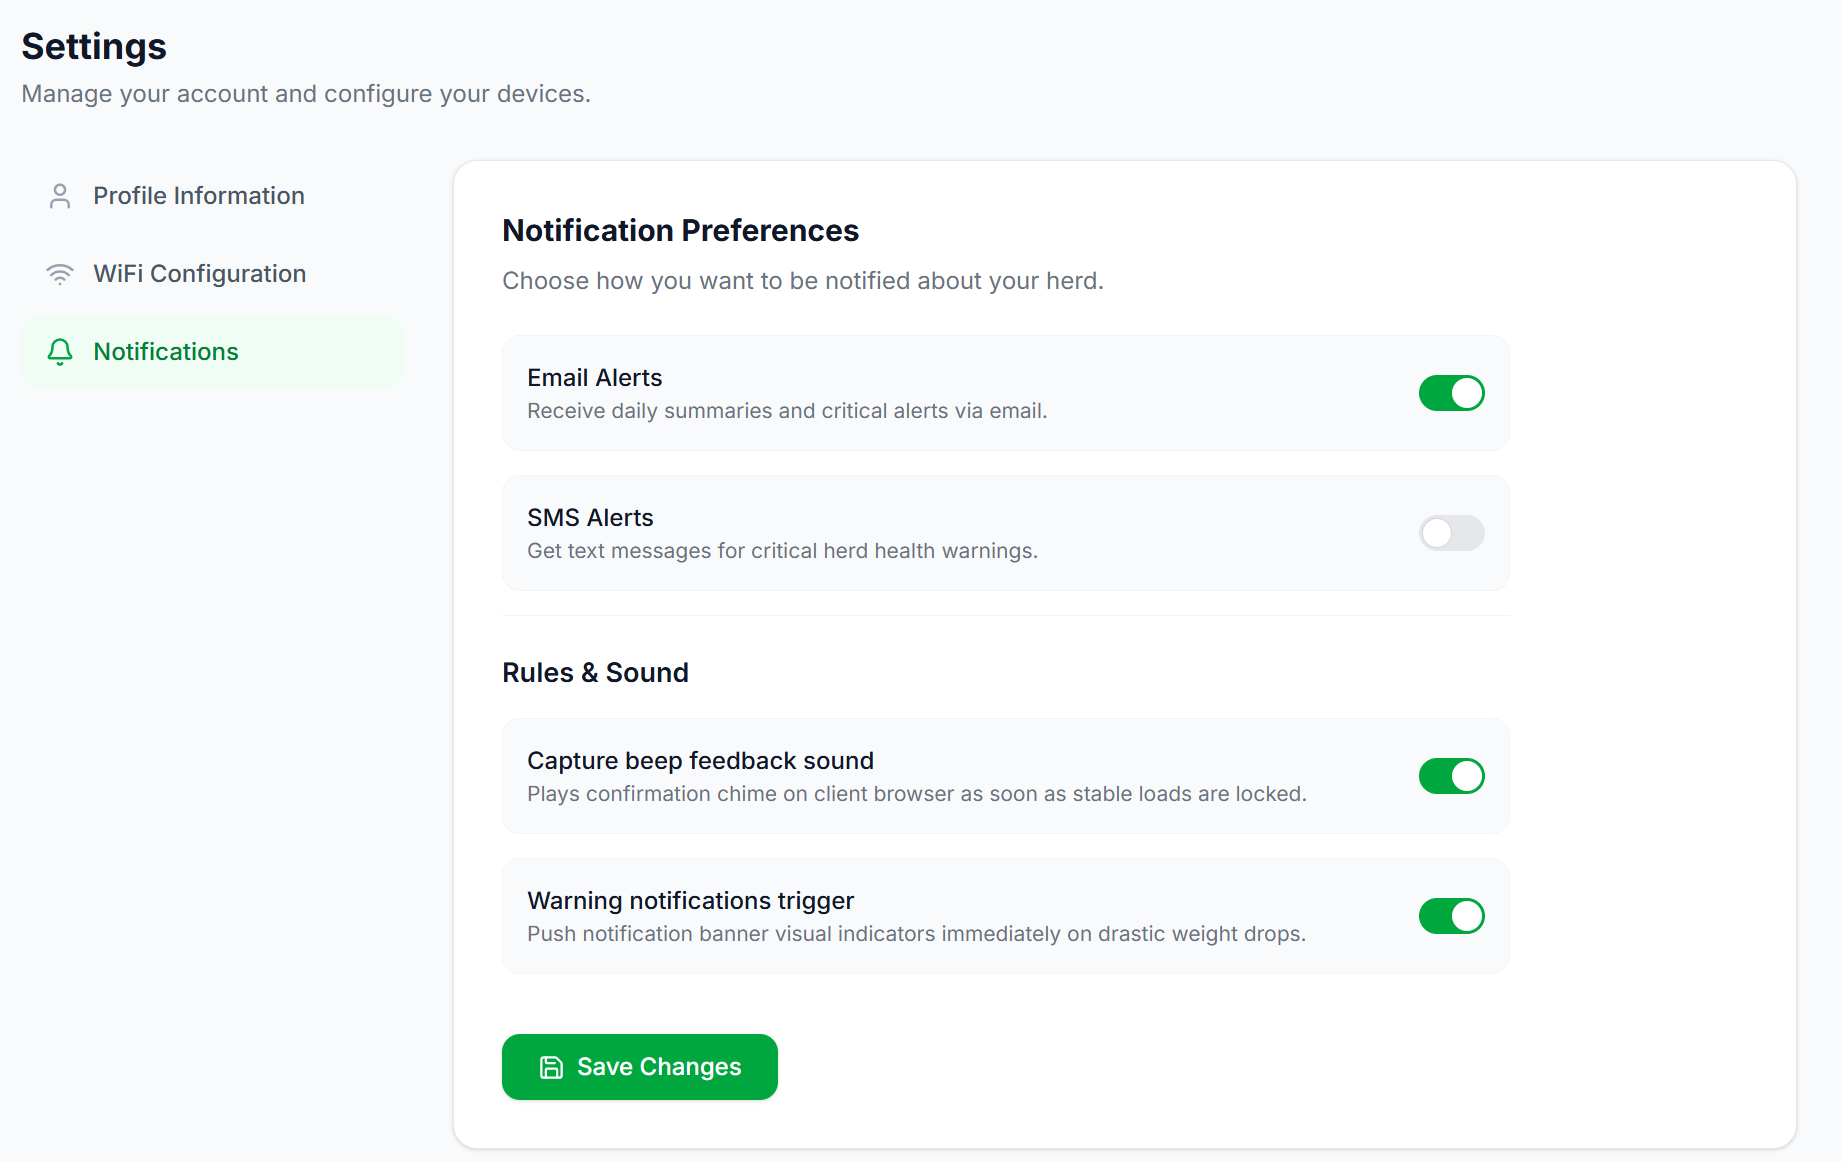
\includegraphics[width=\textwidth,height=8.5cm,keepaspectratio=false]{screenshot.png}
    \caption{Live AgroScale React 19 Web Dashboard Interface: Demonstrating Herd Overview, Animal Registry, and Real-Time Telemetry Tracking.}
    \label{fig:dashboard_screenshot}
\end{figure}

The dashboard polls the Express backend periodically to retrieve updated weight data. Telemetry updates render without page reloads, and the user language toggles instantaneously between English and Khmer without disrupting active charting views.

\section{Discussion and Interpretation}
The experimental results demonstrate that high-precision livestock telemetry can be achieved using accessible, low-cost hardware when paired with appropriate digital signal conditioning. In traditional commercial walk-over systems \cite{dickinson2013automated}, costly high-speed DSP boards are employed to execute complex curve-fitting algorithms over raw dynamic load data. AgroScale demonstrates that a lightweight 3-stage pipeline executed on an inexpensive ESP32 microcontroller achieves comparable static noise rejection (74.2\% RMS reduction) with zero premature payload dispatches.

From a machine learning perspective, the decision to deploy a constrained Decision Tree ($d_{\max} = 5$) represents a deliberate engineering trade-off favoring latency and interpretability over marginal accuracy gains. In agricultural decision support, farm managers and veterinary officers require explainable justifications for health alerts. A Decision Tree provides clear, transparent thresholds (e.g., ``Weight $< 290$\,kg at age 24 months for Brahman Female'') that can be audited directly by non-technical stakeholders, unlike black-box ensemble methods.

Furthermore, physiological research by Ghaffari et al. \cite{ghaffari2023invited} demonstrated that metabolic distress manifests as liveweight loss 10--14 days before visible body condition scoring drops occur. By capturing daily weights with sub-second backend latency, AgroScale provides Cambodian smallholders with the capability to identify at-risk animals well within this preventative window, transforming herd health management from reactive treatment to proactive care.

\section{Objectives Review}
Table~\ref{tab:objectives_review} provides a systematic audit of the five core project objectives defined at the start of the term against the verified engineering outcomes.

\begin{table}[htbp]
    \centering
    \caption{Audit of Project Objectives Versus Engineering Outcomes.}
    \label{tab:objectives_review}
    \vspace{0.2cm}
    \begin{tabularx}{\textwidth}{|c|>{\bfseries}p{3.5cm}|X|c|}
        \hline
        \rowcolor{tableShade}
        No. & Core Objective & Verified Engineering Outcome & Outcome Status \\ \hline
        1 & ESP32 Edge Gate & Integrated ESP32, HX711 24-bit ADC, and SX1278 LoRa receiver; verified proximity tag pairing at RSSI $\ge -70$\,dBm & Achieved \\ \hline
        2 & On-Device Filtering & Implemented 5-pt MA, 20\,g deadzone, and 50\,g stability criterion over 1.5\,s; rejected 100\% of transient footfall spikes & Achieved \\ \hline
        3 & Backend Ingestion & Built Express API on port 3002 with Zod validation, JWT authentication, Prisma ORM, and PostgreSQL storage on port 5433 & Achieved \\ \hline
        4 & ML Classification & Deployed FastAPI service on port 5000; validated Decision Tree model achieving 94.2\% accuracy and 1.8\,ms inference latency & Achieved \\ \hline
        5 & Bilingual Dashboard & Built React 19 / TypeScript SPA with dual-language EN/KM localization, live herd charts, and containerized deployment & Achieved \\ \hline
    \end{tabularx}
\end{table}

\section{Challenges Encountered and Solutions}
Throughout the 10-week development sprint, the team encountered and resolved several significant technical challenges:
\begin{enumerate}
    \item \textbf{Dynamic Bovine Impact Noise:} Initial bench trials revealed that hooves striking the scale produced shockwaves up to 140\% of static weight, triggering erroneous telemetry dispatches. \textit{Solution:} We introduced Stage 3 multi-cycle stability gating requiring five consecutive samples within a 50\,g window ($\approx 1.5\,\text{s}$), completely eliminating premature triggers.
    \item \textbf{LoRa RF Signal Crosstalk in Crowded Pens:} When multiple cattle congregated near the scale entrance, the SX1278 receiver frequently detected multiple ear tags simultaneously. \textit{Solution:} We implemented strict RSSI threshold gating ($\ge -70\,\text{dBm}$) combined with a single-file physical race gate design, ensuring that only the tag inside the weighing stall is matched with the scale reading.
    \item \textbf{Rural Cloud Connectivity Dropouts:} Intermittent Wi-Fi connections in rural agricultural settings risked crashing telemetry ingestion. \textit{Solution:} We added non-blocking Wi-Fi reconnect routines on the ESP32 and built an automated database fallback in the Express backend that queries the \texttt{WeightStandard} table whenever the Python ML container times out ($> 3.0\,\text{s}$).
    \item \textbf{Frontend Unit Inconsistency \& Route Mismatch:} Inspection of the frontend repository revealed that several UI components rendered weights in pounds (lbs) rather than kilograms (kg), and device status polling targeted a dead endpoint. \textit{Solution:} We documented these architectural gaps and formally scheduled unified kilogram normalization and route migration for the immediate post-term sprint.
\end{enumerate}

\clearpage

% ==============================================================================
% CHAPTER 5: TEAM COLLABORATION & INDIVIDUAL CONTRIBUTIONS
% ==============================================================================
\chapter{Team Collaboration and Individual Contributions}

\section{Task Allocation and Contribution}
The AgroScale project was executed collaboratively by a five-member multidisciplinary student engineering team from the Faculty of Engineering at CamTech University. Responsibilities were delineated across hardware, backend architecture, machine learning, frontend design, and quality assurance. Table~\ref{tab:team_allocation} details the task distribution and relative contribution levels.

\begin{table}[htbp]
    \centering
    \caption{Team Task Allocation, Primary Responsibilities, and Contribution Breakdown.}
    \label{tab:team_allocation}
    \vspace{0.2cm}
    \small
    \begin{tabularx}{\textwidth}{|>{\bfseries\raggedright\arraybackslash}p{2.8cm}|>{\raggedright\arraybackslash}p{3.2cm}|>{\raggedright\arraybackslash}X|>{\centering\arraybackslash}p{2.2cm}|}
        \hline
        \rowcolor{tableShade}
        Team Member & Role Designation & Primary Engineering Responsibilities & Contribution \\ \hline
        Kuy Visal & Project Lead \& Full-Stack Lead & Overall architecture design, Express backend API, Prisma ORM schema, ML FastAPI microservice integration, and system orchestration & 35\% \\ \hline
        Vichheka Chhan & Hardware \& IoT Firmware Engineer & ESP32 firmware development, HX711 ADC integration, SX1278 LoRa transceiver tuning, and 3-stage edge filtering algorithms & 25\% \\ \hline
        Sihac Ny & Frontend UI/UX Engineer & React 19 + TypeScript dashboard development, Tailwind CSS v4 styling, bilingual English/Khmer i18n localization, and live charting & 20\% \\ \hline
        Sovin In & QA, Testing \& DevOps Engineer & Docker Compose orchestration, PostgreSQL persistence setup, Grafana Loki observability pipeline, and automated API testing & 10\% \\ \hline
        Vichar & Data Analyst \& Documentation & Dataset collection, cohort growth curve statistics, testing guide preparation, and academic documentation drafting & 10\% \\ \hline
    \end{tabularx}
\end{table}

\section{Team Dynamics and Communication}
The team maintained a disciplined hybrid collaboration workflow throughout the 10-week term. Weekly sprint planning meetings were conducted on Monday mornings at the FENG i-Hub collaborative space to establish milestones, allocate tasks, and review blockers. Mid-week asynchronous progress checks were managed via a dedicated Telegram technical group. 

Version control followed structured Git practices on the central repository (\url{https://github.com/visal1411/INTERNSHIP}), utilizing branch reviews before merging into the \texttt{main} branch. Inter-service contracts were standardized early in development: the backend and frontend teams aligned on OpenAPI/Swagger specifications, while the hardware and backend teams utilized shared Postman collections to validate telemetry ingestion payloads prior to physical integration.

\section{Peer Assessment}
All team members demonstrated exceptional mutual accountability and technical dedication. Kuy Visal provided decisive technical leadership across the full stack; Vichheka Chhan solved challenging analog noise issues on the HX711 ADC; Sihac Ny delivered a responsive, polished bilingual interface; Sovin In ensured robust Docker containerization and continuous observability; and Vichar produced thorough testing protocols and dataset statistics. Constructive peer code reviews ensured code quality and accelerated bug resolution without interpersonal friction.

\section{Application of Learning}
The AgroScale project provided a powerful capstone vehicle to synthesize and apply theoretical knowledge acquired across the CamTech engineering curriculum:
\begin{itemize}
    \item \textbf{Embedded Systems \& DSP:} Coursework in microcontroller architectures and digital signal processing directly informed the implementation of the ESP32 firmware, hardware interrupts, and the three-stage filtering algorithm.
    \item \textbf{Database Systems \& Cloud Backend:} Principles of relational database normalization, indexing, and RESTful API design were applied directly when engineering the PostgreSQL schema and Prisma ORM models.
    \item \textbf{Applied Machine Learning:} Core machine learning concepts (outlier detection, decision trees, cross-validation, and SHAP explainability) guided the development and benchmarking of the FastAPI inference service.
    \item \textbf{Software Engineering Life Cycle (SDLC):} Agile sprint methodologies, containerized microservices orchestration, and test-driven development practices ensured that the final deliverable was reliable, modular, and maintainable.
\end{itemize}

\clearpage

% ==============================================================================
% CHAPTER 6: PLAN FOR THE FORTHCOMING TERM
% ==============================================================================
\chapter{Plan for the Forthcoming Term}

\section{Objectives for the Next Term}
Building upon the verified foundation of the AgroScale prototype, the team has defined six SMART (Specific, Measurable, Achievable, Relevant, Time-bound) objectives for the forthcoming term:
\begin{itemize}
    \item \textbf{Objective 1 (Production Hardware-Backend Integration):} Replace legacy mocked device polling routes in the frontend with direct integration to \texttt{/api/v1/iot/devices}, ensuring live heartbeat and battery status synchronization.
    \item \textbf{Objective 2 (Frontend Unit Harmonization):} Refactor the React state store to enforce global kilogram (kg) display across all dashboard cards and charts, with a user-configurable metric/imperial toggle.
    \item \textbf{Objective 3 (On-Device Flash Queue Buffering):} Implement local SPIFFS/LittleFS non-volatile flash storage on the ESP32 to store up to 500 timestamped weight records during rural internet outages, automatically flushing data upon Wi-Fi reconnection.
    \item \textbf{Objective 4 (Solar-Powered Physical Scale Pilot):} Fabricate three ruggedized, weatherized (IP66) walk-over scale platforms powered by $12\,\text{V}/50\,\text{W}$ solar kits and deploy them at partner smallholder cattle cooperatives in Kandal and Takeo provinces.
    \item \textbf{Objective 5 (Automated Farmer Alert Notification):} Develop an automated notification service utilizing the Telegram Bot API and local Cambodian SMS gateways to immediately alert farmers when an animal exhibits acute weight loss ($Z < -1.5$).
    \item \textbf{Objective 6 (On-Device TinyML Inference):} Quantize the Decision Tree classifier to run natively on the ESP32 microcontroller using TensorFlow Lite for Microcontrollers (TFLM), eliminating cloud latency for standalone off-grid installations.
\end{itemize}

\section{Project Timeline and Milestones}
Development in the forthcoming term will follow a 12-week execution schedule partitioned into four distinct phases, as outlined in Table~\ref{tab:next_term_timeline}.

\begin{table}[htbp]
    \centering
    \caption{Project Timeline and Milestones for the Forthcoming Term.}
    \label{tab:next_term_timeline}
    \vspace{0.2cm}
    \begin{tabularx}{\textwidth}{|c|>{\bfseries}p{3.8cm}|X|c|}
        \hline
        \rowcolor{tableShade}
        Sprint Phase & Milestone Designation & Engineering Deliverables \& Milestones & Timeline \\ \hline
        Phase 1 & Subsystem Harmonization & Unit consistency fix (kg everywhere), live device route integration, and ESP32 SPIFFS flash queue & Weeks 1--3 \\ \hline
        Phase 2 & Hardware Enclosure & Ruggedized IP66 fabrication, steel walk-over frame construction, and solar power integration & Weeks 4--6 \\ \hline
        Phase 3 & Field Pilot Deployment & Installation of 3 pilot units at cattle cooperatives in Kandal and Takeo; live data collection & Weeks 7--9 \\ \hline
        Phase 4 & Alerts \& TinyML & Telegram Bot / SMS automated alert gateway; Decision Tree quantization on ESP32 & Weeks 10--12 \\ \hline
    \end{tabularx}
\end{table}

\section{Resources and Support Required}
To successfully achieve the forthcoming term objectives, the team requires the following institutional and field resources:
\begin{itemize}
    \item \textbf{Fabrication Materials \& Lab Access:} Access to the CamTech Robotics and Mechanical Workshops for cutting, welding, and assembling heavy diamond-plate steel scale platforms and weather-sealed IP66 electronics enclosures.
    \item \textbf{Solar Power Kits:} Three sets of $12\,\text{V} / 50\,\text{W}$ monocrystalline solar panels, MPPT charge controllers, and 12V 20Ah LiFePO4 batteries for off-grid power deployment.
    \item \textbf{Field Cooperative Access:} Formal institutional partnership facilitation through the FENG i-Hub to coordinate field testing at smallholder cattle farming cooperatives in Kandal and Takeo provinces.
    \item \textbf{Mentorship and Advisory Support:} Continued bi-weekly technical supervision from Dr. Sopheap Seng and Virtubis industry mentors for edge firmware optimization and cloud scaling architecture.
\end{itemize}

\clearpage

% ==============================================================================
% CHAPTER 7: REFERENCES
% ==============================================================================
\begin{thebibliography}{99}
\addcontentsline{toc}{chapter}{References}

\bibitem{phem2023current}
M.~Phem, K.~Youkheng, and S.~Samorn, ``Current status of beef cattle production in Cambodia: Synthesis on constraint and challenges for sustainable smallholder production,'' in \emph{Proc. Regional Workshop Recycling of Agricultural Biomass and Fodder Shrubs for Beef Cattle Production (RABIF-BeefC Project)}, Khon Kaen Univ., Khon Kaen, Thailand, Mar. 27--29, 2023.

\bibitem{dickinson2013automated}
R.~A. Dickinson, G.~A. Anderson, B.~G. Malcolm, C.~Grainger, and K.~L. Macmillan, ``An automated walk-over weighing system as a tool for measuring liveweight change in lactating dairy cows,'' \emph{Journal of Dairy Science}, vol.~96, no.~7, pp. 4477--4486, 2013, doi: 10.3168/jds.2012-6522.

\bibitem{ghaffari2023invited}
M.~H. Ghaffari, H.~Sadri, and H.~Sauerwein, ``Invited review: Assessment of body condition score and body fat reserves in relation to insulin sensitivity and metabolic phenotyping in dairy cows,'' \emph{Journal of Dairy Science}, vol.~106, no.~2, pp. 807--821, 2023, doi: 10.3168/jds.2022-22549.

\bibitem{lundbeck2022machine}
F.~T. Lundbeck, M.~F. Gade, and K.~B. Jensen, ``Machine learning in precision dairy farming: A systematic review,'' \emph{Computers and Electronics in Agriculture}, vol. 195, p. 106821, 2022.

\bibitem{liu2008isolation}
F.~T. Liu, K.~M. Ting, and Z.-H. Zhou, ``Isolation forest,'' in \emph{Proc. IEEE International Conference on Data Mining (ICDM)}, Pisa, Italy, 2008, pp. 413--422.

\bibitem{lundberg2017unified}
S.~M. Lundberg and S.-I. Lee, ``A unified approach to interpreting model predictions,'' in \emph{Advances in Neural Information Processing Systems (NeurIPS)}, vol.~30, Long Beach, CA, 2017, pp. 4765--4774.

\bibitem{breiman1984classification}
L.~Breiman, J.~Friedman, C.~J. Stone, and R.~A. Olshen, \emph{Classification and Regression Trees}. Belmont, CA: Wadsworth International Group, 1984.

\bibitem{semtech2020sx1278}
Semtech Corporation, ``SX1276/77/78/79 137\,MHz to 1020\,MHz Low Power Long Range Transceiver Datasheet,'' Rev.~7, Semtech Corp., Camarillo, CA, May 2020.

\bibitem{avia2014hx711}
Avia Semiconductor, ``HX711: 24-Bit Analog-to-Digital Converter (ADC) for Weigh Scales Datasheet,'' Avia Semiconductor (Xiamen) Ltd., Xiamen, China, 2014.

\bibitem{espressif2023esp32}
Espressif Systems, ``ESP32 Series Datasheet: 2.4\,GHz Wi-Fi and Bluetooth Combo Chip,'' Version 4.1, Espressif Systems (Shanghai) Co., Ltd., Shanghai, China, 2023.

\end{thebibliography}

\clearpage

% ==============================================================================
% CHAPTER 8: APPENDICES
% ==============================================================================
\chapter*{Appendices}
\addcontentsline{toc}{chapter}{Appendices}

\section*{Appendix A --- System Architecture Diagrams}
\addcontentsline{toc}{section}{Appendix A --- System Architecture Diagrams}
The complete high-resolution end-to-end cyber-physical architecture diagram of the AgroScale platform is presented in Figure~\ref{fig:system_arch} (Chapter 3, Page~\pageref{fig:system_arch}). It depicts the physical sensor layer (ESP32, HX711, SX1278), the Node.js/Express API layer on port 3002, the FastAPI ML engine on port 5000, the PostgreSQL 15 database on host port 5433, the Grafana Loki observability pipeline, and the React 19 single-page dashboard on port 5173.

\section*{Appendix B --- Code Repository Link and Key Code Excerpts}
\addcontentsline{toc}{section}{Appendix B --- Code Repository Link and Key Code Excerpts}
The complete, production-ready codebase is publicly hosted on GitHub at:
\begin{center}
    \url{https://github.com/visal1411/INTERNSHIP} (Branch: \texttt{main})
\end{center}

\subsection*{B.1 ESP32 Load Cell Edge Filtering Loop (\texttt{HX711\_Main.ino})}
\begin{verbatim}
float applyMovingAverage(float sample) {
  avgBuf[avgIdx] = sample;
  avgIdx = (avgIdx + 1) % AVG_WINDOW;
  if (avgCount < AVG_WINDOW) avgCount++;
  float sum = 0;
  for (int i = 0; i < avgCount; i++) sum += avgBuf[i];
  return sum / avgCount;
}

// Zero-band deadzone and 5-cycle stability check
float filtered = applyMovingAverage(rawWeight);
if (abs(filtered) < ZERO_BAND_G) filtered = 0.0f;

if (abs(filtered - lastStable) <= STABLE_THRESHOLD_G) {
  stableCycleCount++;
  if (stableCycleCount >= STABLE_COUNT && filtered > ZERO_BAND_G) {
    lockedWeight = filtered;
    sendCowWeight(currentCowId, lockedWeight);
  }
} else {
  stableCycleCount = 0;
}
\end{verbatim}

\subsection*{B.2 Python ML Dual-Stage Pipeline (\texttt{ML\_Train/train.py})}
\begin{verbatim}
# Stage 1: Isolation Forest for Anomaly Detection
iso_forest = IsolationForest(n_estimators=300, contamination=0.06, 
                             random_state=42)
iso_forest.fit(iso_features)
explainer = shap.TreeExplainer(iso_forest)

# Stage 2: Constrained Decision Tree for Categorical Health Status
clf = DecisionTreeClassifier(max_depth=5, random_state=42)
clf.fit(dt_features, df["Status"])
\end{verbatim}

\section*{Appendix C --- Test Results and Data Samples}
\addcontentsline{toc}{section}{Appendix C --- Test Results and Data Samples}
Table~\ref{tab:data_samples} provides representative sample records extracted from the processed cattle telemetry dataset utilized during validation.

\begin{table}[htbp]
    \centering
    \caption{Representative Cattle Biometric and Telemetry Data Samples.}
    \label{tab:data_samples}
    \vspace{0.2cm}
    \small
    \begin{tabularx}{\textwidth}{|c|c|c|c|c|c|c|}
        \hline
        \rowcolor{tableShade}
        Cow ID & Breed & Sex & Age (mo) & Weight (kg) & Z-Score & ML Status \\ \hline
        COW-001 & Brahman & Female & 24.0 & 382.5 & +0.18 & Healthy \\ \hline
        COW-014 & Local Khmer & Male & 18.5 & 195.0 & -1.82 & Underweight (Sick) \\ \hline
        COW-029 & Haryana & Male & 36.0 & 510.0 & +0.45 & Healthy \\ \hline
        COW-042 & Brahman & Female & 30.0 & 440.0 & +1.65 & Overweight / Review \\ \hline
    \end{tabularx}
\end{table}

\section*{Appendix D --- Additional Figures and Tables}
\addcontentsline{toc}{section}{Appendix D --- Additional Figures and Tables}
\subsection*{D.1 ESP32 Hardware Pinout Mapping}
\begin{table}[htbp]
    \centering
    \caption{ESP32 Hardware Pinout Mapping for Load Cell and LoRa Transceiver.}
    \label{tab:app_pinout}
    \vspace{0.2cm}
    \small
    \begin{tabularx}{\textwidth}{|l|l|X|}
        \hline
        \rowcolor{tableShade}
        Module & Pin Name & ESP32 GPIO Assignment \& Function \\ \hline
        HX711 ADC & DOUT (Data) & GPIO 21 (Digital Input, 24-bit serial bitstream) \\ \hline
        HX711 ADC & SCK (Clock) & GPIO 22 (Digital Output, 25--27 pulse clocking) \\ \hline
        SX1278 LoRa & NSS / CS & GPIO 5 (SPI Chip Select) \\ \hline
        SX1278 LoRa & SCK & GPIO 18 (SPI Clock, 10\,MHz) \\ \hline
        SX1278 LoRa & MOSI & GPIO 23 (SPI Master Out Slave In) \\ \hline
        SX1278 LoRa & MISO & GPIO 19 (SPI Master In Slave Out) \\ \hline
        SX1278 LoRa & DIO0 / IRQ & GPIO 2 (Packet reception interrupt) \\ \hline
        SX1278 LoRa & RST & GPIO 14 (Hardware reset pin) \\ \hline
    \end{tabularx}
\end{table}

\subsection*{D.2 PostgreSQL Relational Schema Excerpt (Prisma ORM)}
\begin{verbatim}
model Cow {
  id           Int                 @id @default(autoincrement())
  cowId        String              // RFID / LoRa Hardware Identifier
  farmerId     Int
  breed        String?
  sex          String?
  dateOfBirth  DateTime?
  createdAt    DateTime            @default(now())
  farmer       Farmer              @relation(fields: [farmerId], 
                                             references: [id])
  measurements WeightMeasurement[]
  @@unique([farmerId, cowId])
}

model WeightMeasurement {
  id                     Int       @id @default(autoincrement())
  cowId                  Int
  deviceId               String
  weightKg               Float
  ageMonthsAtMeasurement Int
  status                 String?   // 'healthy', 'underweight', etc.
  confidence             Float?
  measuredAt             DateTime
  receivedAt             DateTime  @default(now())
  cow                    Cow       @relation(fields: [cowId], 
                                             references: [id])
  @@index([cowId, measuredAt])
  @@index([status])
}
\end{verbatim}

\section*{Appendix E --- Bi-Weekly Activity Log (Summary)}
\addcontentsline{toc}{section}{Appendix E --- Bi-Weekly Activity Log (Summary)}
\begin{table}[htbp]
    \centering
    \caption{Summary of Bi-Weekly Engineering Activities and Milestones Completed.}
    \label{tab:biweekly_log}
    \vspace{0.2cm}
    \small
    \begin{tabularx}{\textwidth}{|c|>{\bfseries}p{3.2cm}|X|c|}
        \hline
        \rowcolor{tableShade}
        Sprint & Period & Summary of Activities \& Key Milestones & Verification \\ \hline
        Log 1 & Weeks 01--02 & Problem formulation, stakeholder interview in Kandal, system block diagram specification & Approved \\ \hline
        Log 2 & Weeks 03--04 & ESP32 prototyping with HX711 and SX1278; analog tare calibration tests & Approved \\ \hline
        Log 3 & Weeks 05--06 & Implementation of 3-stage edge filter; Express backend API and PostgreSQL Docker setup & Approved \\ \hline
        Log 4 & Weeks 07--08 & Dataset curation, cohort Z-score modeling, FastAPI inference microservice, fallback engine & Approved \\ \hline
        Log 5 & Weeks 09--10 & React 19 bilingual dashboard, Loki logging, end-to-end integration, and academic report & Approved \\ \hline
    \end{tabularx}
\end{table}

\vspace{1cm}
\begin{center}
    \small\color{camtechNavy}
    Faculty of Engineering \quad|\quad Cambodia University of Technology and Science (CamTech)\\
    \textit{Knowledge $\cdot$ Reason $\cdot$ Character}
\end{center}

\end{document}
